\documentclass{beamer}


\title{(a, b) and B-Trees}
\author{%
    Martín Hernández\\%
    Juan Mendivelso%
}
\date{} % Empty Date

% Libraries / Packages
\usepackage{graphicx} % Required for inserting images
\usepackage{biblatex}
    \addbibresource{resources/bibliography.bib}
\usepackage{listings}
\usepackage{csquotes}
\usepackage{wrapfig}
\usepackage{mathtools}
\usepackage{unicode-math}

% Template
\NewDocumentCommand{\shortauthors}{}{%
    Hernández, %
    Mendivelso%
}
% Listings code env and inline stuff
\lstset{%
basicstyle=\ttfamily%
}

\lstdefinestyle{codeinc}{%
    escapechar=\%,%
    numbers=left,%
    stepnumber=1,%
    tabsize=1,%
    commentstyle=\color{gray},%
    basicstyle=\small,%
    breaklines=true,%
    language=C%
}

% Text
\setbeamercolor{titlelike}{fg=black}
\setbeamerfont{titlelike}{size=\Large,series=\bfseries}

\setbeamerfont{title}{series=\bfseries,size=\huge}
\setbeamerfont{structure}{series=\bfseries,size=\large}
\setbeamercolor{structure}{fg=black}

\setbeamercolor{footline}{fg=gray}
\setbeamerfont{footline}{size*={4.5}{-1}}
\setbeamerfont{framenumber}{size*={8}{0}}

% Frame columns sizes

\newcommand{\textlecolumn}{0.9\textwidth}
\newcommand{\textricolumn}{0.1\textwidth}

% Footline
\setbeamertemplate{navigation symbols}{}
\setbeamertemplate{footline}{%
    \hbox{%
        \begin{beamercolorbox}[wd=1\paperwidth,dp=2.5ex,right]{framenumber}%
            \usebeamerfont{framenumber}
            \insertframenumber{}%
            \hspace*{2ex}%
        \end{beamercolorbox}
    }%
    \vskip0pt%
    %
    \begin{center}%
        \vspace{-4mm}
        Presentation made by \shortauthors{}. Contents and figures extracted from the book: Advanced Data Structures. Peter Brass. Cambridge University Press. 2008.
        \vspace{-3mm}
    \end{center}%
%
}

\begin{document}
% Code elemenst definitions
\defverbatim[colored] \btreeStructure {%
\begin{lstlisting}[style=codeinc]
int alpha = 2 /* any int >= 2 */
typedef struct tr_n_t {
  int degree;
  int height;
  key_t key[2 * alpha];
  struct tr_n_t * next[(2 * alpha) + 1];
  /* possibly other information */
} tree_node_t;
\end{lstlisting}
}

\defverbatim[colored] \btreeCreateEmpty {%
\begin{lstlisting}[style=codeinc]
tree_node_t *create_tree(){ 
  tree_node_t *tmp;
  tmp = get_node();
  tmp->height = 0;
  tmp->degree = 0;
  return( tmp );
}
\end{lstlisting}
}

\defverbatim[colored] \btreeSearch {%
\begin{lstlisting}[style=codeinc]
object_t *find(tree_node_t *tree, key_t query_key) { 
  tree_node_t *current_node;
  object_t *object;
  current_node = tree;
  while( current_node->height >= 0 ) { /* binary search among keys */
    int lower, upper;
    lower = 0;
    upper = current_node->degree;
    while( upper > lower +1 ) {
      if( query_key < current_node->key[(upper+lower)/2 ] )
        upper = (upper+lower)/2;
      else
        lower = (upper+lower)/2;
    }
    if( current_node->height > 0)
      current_node = current_node->next[lower + 1]; /* Offset sub-tree ptrs def */
    else { /* block of height 0, contains the object pointers */
      if( current_node->key[lower] == query_key )
        object = (object_t *)
        current_node->next[lower];
      else
        object = NULL;
      return( object );
    }
  }
}
\end{lstlisting}
}

\defverbatim[colored] \btreeDestroy {%
\begin{lstlisting}[style=codeinc]
void btDestroy(bTree b) {
  if(!b->isLeaf) {
    for (int i = 0; i < b->numKeys + 1; i++) {
      btDestroy(b->kids[i]);
    }
  }
  free(b);
}
\end{lstlisting}
}

\defverbatim[colored] \btreeSearchStepOne {%
\begin{lstlisting}[style=codeinc,numbers=none]
query_key = 16;
tree = *(node 1);

object = NULL;
current_node = *(node 1);
current_node->height = 1;
current_node->degree = 2;

lower = 0;
upper = 2;
\end{lstlisting}
}

\defverbatim[colored] \btreeSearchStepTwo {%
\begin{lstlisting}[style=codeinc,numbers=none]
query_key = 16;
tree = *(node 1);

object = NULL;
current_node = *(node 1);
current_node->height = 1;
current_node->degree = 2;

lower = 2; 
upper = 2;
\end{lstlisting}
}

\defverbatim[colored] \btreeSearchStepThree {%
\begin{lstlisting}[style=codeinc,numbers=none]
query_key = 16;
tree = *(node 1);

object = NULL;
current_node = *(node 5);
current_node->height = 0;
current_node->degree = 3;

lower = 0; 
upper = 3;
\end{lstlisting}
}

\defverbatim[colored] \btreeSearchStepFour {%
\begin{lstlisting}[style=codeinc,numbers=none]
query_key = 16;
tree = *(node 1);

object = NULL;
current_node = *(node 5);
current_node->height = 0;
current_node->degree = 3;

lower = 0; 
upper = 2;
\end{lstlisting}
}

\defverbatim[colored] \btreeSearchStepFive {%
\begin{lstlisting}[style=codeinc,numbers=none]
query_key = 16;
tree = *(node 1);

object = NULL;
current_node = *(node 5);
current_node->height = 0;
current_node->degree = 3;

lower = 0; 
upper = 1;
\end{lstlisting}
}

\defverbatim[colored] \btreeSearchStepSix {%
\begin{lstlisting}[style=codeinc,numbers=none]
query_key = 16;
tree = *(node 1);

object = *(16);
current_node = *(node 5);
current_node->height = 0;
current_node->degree = 3;
\end{lstlisting}
}

\defverbatim[colored] \btreeSearchStepSeven {%
\begin{lstlisting}[style=codeinc,numbers=none]
query_key = 16;
tree = *(node 1);

object = NULL;
current_node = *(node 5);
current_node->height = 0;
current_node->degree = 3;
\end{lstlisting}
}

\defverbatim[colored] \btreeInsert {%
\begin{lstlisting}[style=codeinc]
void btInsert(bTree b, int key) {
  bTree b1, b2;
  int median;

  b2 = btInsertInternal(b, key, &median);
  if(!b2) {
    return;
  }
  
  b1 = malloc(sizeof(*b1));
  memmove(b1, b, sizeof(*b));
  b->numKeys = 1;
  b->isLeaf = 0;
  b->keys[0] = median;
  b->kids[0] = b1;
  b->kids[1] = b2;
}
\end{lstlisting}
}

\defverbatim[colored] \btreeInsertInternalPartOne {%
\begin{lstlisting}[style=codeinc]
bTree btInsertInternal(bTree b, int key, int *median) {
  int pos = searchKey(b->numKeys, b->keys, key);
  int mid;
  bTree b2;

  if(pos < b->numKeys && b->keys[pos] == key)
    return 0; /* nothing to do */

  if(b->isLeaf) { 
      memmove(&b->keys[pos+1], &b->keys[pos], sizeof(*(b->keys)) * (b->numKeys - pos));
      b->keys[pos] = key;
      b->numKeys++;
  } else {
    ...
\end{lstlisting}
}

\defverbatim[colored] \btreeInsertInternalPartTwo {%
\begin{lstlisting}[style=codeinc,firstnumber=12]
    ...
  } else {
    b2 = btInsertInternal(b->kids[pos], key, &mid);      
    if(b2) {
      memmove(&b->keys[pos+1], &b->keys[pos], sizeof(*(b->keys)) * (b->numKeys - pos));
      memmove(&b->kids[pos+2], &b->kids[pos+1], sizeof(*(b->keys)) * (b->numKeys - pos));

      b->keys[pos] = mid;
      b->kids[pos+1] = b2;
      b->numKeys++;
    }
  }
\end{lstlisting}
}

\defverbatim[colored] \btreeInsertInternalPartThree {%
\begin{lstlisting}[style=codeinc,firstnumber=24]
  ...
  if(b->numKeys >= (2*alpha - 1)) {
    mid = b->numKeys/2;

    *median = b->keys[mid];

    /* make a new node for keys > median */
    b2 = malloc(sizeof(*b2));

    b2->numKeys = b->numKeys - mid - 1;
    b2->isLeaf = b->isLeaf;

    memmove(b2->keys, &b->keys[mid+1], sizeof(*(b->keys)) * b2->numKeys);
    if(!b->isLeaf) {
        memmove(b2->kids, &b->kids[mid+1], sizeof(*(b->kids)) * (b2->numKeys + 1));
    }

    b->numKeys = mid;
    return b2;  
  } else {
    return 0;
  }
}
\end{lstlisting}
}


\begin{frame}
    \titlepage
\end{frame}

\begin{frame}[allowframebreaks,allowdisplaybreaks]
    \frametitle{Contents}
    \tableofcontents
\end{frame}

\begin{frame}
    \section{Similarities in (a,b)-Trees and B-Trees}
    \frametitle{Similarities in (a,b)-Trees and B-Trees}
    \begin{columns}[T]
        \begin{column}{.55\textwidth}
            \begin{block}{}
                \begin{itemize}
                    \item Both types of trees have higher degree than the previous trees.
                    \item Meaning that, both have more than 1 key and 2 sub-trees in each node.
                    \item Each type has a lower and upper limit of keys and sub-trees, 
                        which are defined by constants.
                    \item Due to the higher degree, there's changes in the code of the
                        \lstinline|find|, \lstinline|insert| and \lstinline|delete| operations.
                \end{itemize}
            \end{block}
        \end{column}
        \begin{column}{.6\textwidth}
            \begin{block}{}
                \begin{figure}
                    \centering
                    \includegraphics[width=\textwidth]{resources/book/ab_tree.png}
                    \caption[]{(a,b)-Tree}
                    \label{ab_tree}
                \end{figure}
            \end{block}
        \end{column}
    \end{columns}    
\end{frame}
\begin{frame}
    \section{B-Tree}
    \subsection{History}
    \frametitle{B-Tree History I}
    \begin{columns}
        \begin{column}{0.5\textwidth}
            \begin{block}{}
                B-Trees where firstly studied, defined and implemented by R. Bayer and E. McCreight in 1972, using an IBM 360 series model 44 with an 2311 disk drive.
                \begin{figure}
                    \centering
                    \includegraphics[width=0.5\textwidth,height=\textheight,keepaspectratio]{resources/made/ibm360_44.png}
                    \caption[]{IBM 360 / 44}
                \end{figure}
            \end{block}
        \end{column}
        \begin{column}{0.5\textwidth}
            \begin{block}{}
                An IBM 360 series model 44 had from 32 to 256 \(KB\) of Random Access Memory, and weighed from 1,315 to 1,905 kg.
                \begin{figure}
                    \centering
                    \includegraphics[width=0.5\textwidth,height=\textheight,keepaspectratio]{resources/made/ibmdisk_2311.png}
                    \caption[]{IBM 2311 disk drive}
                \end{figure}
            \end{block}
        \end{column}
    \end{columns}
\end{frame}
\begin{frame}
    \frametitle{B-Tree History II}
    \begin{columns}
        \begin{column}{0.5\textwidth}
            \begin{block}{}
                \blockquote[Bayer and McCreight]{(\ldots) actual experiments show that it is possible to maintain an index of size 15.000 with an average of 9 retrievals, insertions, and deletions per second in real time on an IBM 360/44 with a 2311 disc as backup store. (\ldots) it should be possible to main tain all index of size 1'500.000 with at least two transactions per second.}
            \end{block}
        \end{column}
        \begin{column}{0.5\textwidth}
            \begin{block}{}
                \begin{figure}
                    \centering
                    \includegraphics[width=0.5\textwidth,height=\textheight,keepaspectratio]{resources/made/ibm360_44.png}
                    \caption[]{IBM 360 / 44}
                \end{figure}
            \end{block}
        \end{column}
    \end{columns}
\end{frame}
\begin{frame}
    \subsection{Definition}
    \frametitle{B-Tree Definition}
    \begin{columns}
        \begin{column}{\textlecolumn}
            \begin{block}{}
                \begin{itemize}
                    \item We will define that \(T\), an object, is a B-Tree if they are an instance of the class.
                    \[
                        T \in t\left(\alpha, h\right)
                    \]
                    \item Where \(h\) is the height of the B-Tree.
                    \item And, \(\alpha\) is a predefined constant.
                \end{itemize}
            \end{block}
        \end{column}
        \begin{column}{\textricolumn}
        \end{column}
    \end{columns}
\end{frame}
\begin{frame}
    \subsection{Properties}
    \subsubsection{The \(\alpha\) Constant}
    \frametitle{B-Tree Properties - The \(\alpha\) constant I}
    \begin{columns}
        \begin{column}{\textlecolumn}
            \begin{block}{}
                \begin{itemize}
                    \item The main property of the B-Trees is the \(\alpha\), a predefined constant.
                    \item This constant will determine the interval of keys and sub-trees, in a balanced node. This is called the \emph{Branching factor} of the tree.
                    \item The tree is balanced if they have from \(\alpha + 1\) to \(2\alpha + 1\) sub-trees in a single node.
                    \item Also, each balanced node have from \(\alpha\) to \(2\alpha\) keys.
                    \item The only node that can have less than \(\alpha + 1\) sub-trees and only 1 key is the root of the tree. 
                    \item But, the root still have the upper bounds of sub-trees and keys.
                \end{itemize}
            \end{block}
        \end{column}
        \begin{column}{\textricolumn}
        \end{column}
    \end{columns}
\end{frame}
\begin{frame}
    \frametitle{B-Tree Properties - The \(\alpha\) constant II}
    \begin{columns}
        \begin{column}{\textlecolumn}
            \begin{block}{}
                \begin{itemize}
                    \item The \(\alpha\) must be a Natural number, \(\alpha \in \mathbb{N}\).
                    \item Since, there's other definitions of B-Trees that define the bounds for the keys and sub-trees in a node differently, generally we choose an \(\alpha \geq 2\).
                    \item Also, the \(\alpha\) is often the greatest number possible that the primary memory can handle the mentioned intervals.
                \end{itemize}
            \end{block}
        \end{column}
        \begin{column}{\textricolumn}
        \end{column}
    \end{columns}
\end{frame}
\begin{frame}
    \frametitle{B-Tree Properties - The \(\alpha\) constant III}
    \begin{columns}
        \begin{column}{\textwidth}
            \begin{block}{}
                \begin{figure}
                    \centering
                    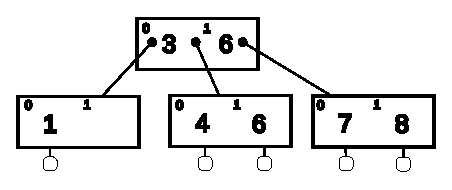
\includegraphics[width=0.65\linewidth,keepaspectratio]{resources/made/a2_btree.eps}
                    \caption[]{B-Tree, t(1, 2)}
                \end{figure}
                \vspace{-0.75cm}
                \begin{figure}
                    \centering
                    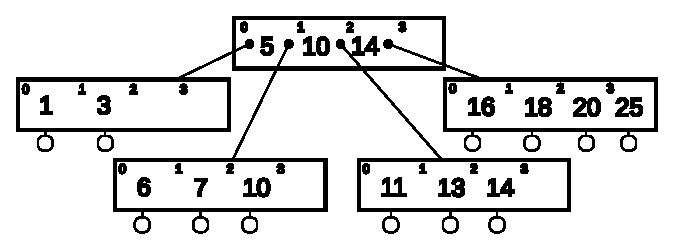
\includegraphics[width=0.75\linewidth,keepaspectratio]{resources/made/a3_btree.eps}
                    \caption[]{B-Tree, t(2, 2)}
                \end{figure}
            \end{block}    
        \end{column}
        \begin{column}{0pt}
        \end{column}
    \end{columns}
\end{frame}
\begin{frame}
    \frametitle{B-Tree Properties - The \(\alpha\) constant IV}
    \begin{columns}
        \begin{column}{\textlecolumn}
            \begin{block}{}
                \vspace{-0.5cm}
                \begin{itemize}
                    \item We can prove the bounds of the number of sub-trees in a node, and define a function that let us get the number of sub-trees in a node.
                \end{itemize}
                \begin{proof}\renewcommand{\qedsymbol}{}
                    Let \(N()\) be a function that takes a B-Tree as an argument and returns the number of nodes in it.
                    \\
                    Let \(N_{min}\) and \(N_{max}\) the minimum and maximal number of nodes in a B-Tree \(T \in t\left(\alpha, h\right)\). Then
                    \[
                        \begin{aligned}
                            N_{min} &= 1 + 2\left(\left(\alpha + 1\right)^0 + \left(\alpha + 1\right)^1 + \cdots + \left(\alpha + 1\right)^{h-2} \right) \\
                            & = 1 + 2\left(\sum^{h - 2}_{i = 0} \left(\alpha + 1\right)^i \right) \\
                            & = 1 + \frac{2}{\alpha}\left(\left(\alpha + 1\right)^{h - 1} - 1\right)
                        \end{aligned}
                    \]
                \end{proof}
            \end{block}
        \end{column}
        \begin{column}{\textricolumn}
        \end{column}
    \end{columns}
\end{frame}
\begin{frame}
    \frametitle{B-Tree Properties - The \(\alpha\) constant V}
    \begin{columns}
        \begin{column}{\textlecolumn}
            \begin{block}{}
                \begin{proof}[\unskip\nopunct]
                    For \(h \geq 1\), we also have that
                    \[
                        \begin{aligned}
                            N_{max} &= 1 + 2\left(\sum^{h - 1}_{i = 0} \left(2\alpha + 1\right)^i \right) \\
                            &= 1 + \frac{1}{2\alpha}\left(\left(2\alpha + 1\right)^{h} - 1\right)
                        \end{aligned}
                    \]
                    \\
                    Then, if \(h = 0\), we have that \(N\left(T\right) = 0\). Else, if \(h \geq 1\)
                    \[
                        1 + \frac{2}{\alpha}\left(\left(\alpha + 1\right)^{h - 1} - 1\right) \leq N\left(T\right) \leq 1 + \frac{1}{2\alpha}\left(\left(2\alpha + 1\right)^{h} - 1\right)
                    \]
                \end{proof}
            \end{block}
        \end{column}
        \begin{column}{\textricolumn}
        \end{column}
    \end{columns}
\end{frame}
\begin{frame}
    \subsubsection{Keys and Sub-trees}
    \frametitle{B-Tree Properties - Keys and Sub-trees}
    \begin{columns}
        \begin{column}{\textlecolumn}
            \begin{block}{}
                \vspace{-0.75cm}
                \begin{itemize}
                    \item The keys and sub-trees are stored in a sequential increasing order.
                    \item We can define \(\symit{l}\) as the number of keys in a node \(N\), which isn't a leaf or root.
                    \item Such that for \(t\left(\alpha, h\right)\), we have \(\alpha \leq \symit{l} \leq 2\alpha\).
                    \item We can consider the sub-trees as \(p_0, p_1, \ldots, p_j\), where \(j\) is the number of sub-trees in \(N\).
                    \item Since there's a sub-tree before and after each key in \(N\).
                    \item Then, \(j\) must be equal to \(\symit{l} + 1\).
                \end{itemize}
            \end{block}
        \end{column}
        \begin{column}{\textricolumn}
            \begin{block}{}
            \end{block}
        \end{column}
    \end{columns}
    \begin{figure}[h!]
        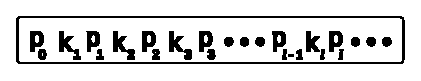
\includegraphics[width=\linewidth]{resources/made/key_subtree_order.eps}
        \caption{Order of Keys and Sub-trees in a B-Tree Node}
    \end{figure}
\end{frame}
\begin{frame}
    \subsubsection{Height and Number of Nodes}
    \frametitle{B-Tree Properties - Height and Number of Nodes}
    \begin{itemize}
        \item The height of a B-Tree \(T\) with \(n \geq 1\) keys and a \(\alpha \geq 2\) is going to be:
    \end{itemize}
    \[
        h \leq log_{\alpha} \frac{n + 1}{2}
    \]
    \begin{proof}\renewcommand{\qedsymbol}{}
        By definition, the \emph{Root} of \(T\) has at least one key if the tree isn't empty. Then, the sub-trees contain at least \(\alpha - 1\) elements. Thus, from the \emph{Root} we have at least \(2\) nodes with a depth of \(1\), then in these nodes we have at least \(2\alpha^{1}\) nodes with a depth of \(2\). We can see that, in the sub-tree \(i\) we are going to have \(2\alpha^{i-1}\) nodes with a depth of \(i + 1\). 
    \end{proof}
    \begin{proof}[\unskip\nopunct]
        We sum the number of nodes from the nodes with depth of 1 all the way to the nodes that have the same depth as the height of the tree, and compare them to the number of keys, which will be greater or equal by definition. Having that:
        \[
            \begin{aligned}
                n &\geq 1 + \left(\alpha - 1\right) \sum_{i = 1}^{h} 2\alpha^{i - 1} \\
                &= 1 + 2\left(\alpha - 1\right)\left(\frac{\alpha^{h} - 1}{\alpha - 1}\right) \\
                &= 2\alpha^h - 1 \\
                \frac{n + 1}{2} &\geq \alpha^h \\
                h &\leq log_{\alpha} \frac{n + 1}{2}
            \end{aligned}
        \]
    \end{proof}
\end{frame}
\begin{frame}
    \subsection{Structure}
    \frametitle{B-Tree Structure}
    \begin{columns}
        \begin{column}{\textlecolumn}
            \begin{block}{}
                \begin{itemize}
                    \item The structure of the B-Tree's node adds two arrays where the keys and sub-trees' pointers will be stored:
                \end{itemize}
            \end{block}
            \begin{block}
                \btreeStructure
            \end{block}
        \end{column}
        \begin{column}{\textricolumn}
        \end{column}
    \end{columns}
\end{frame}
\begin{frame}
    \subsection{Operations}
    \frametitle{B-Tree Operations}
    \begin{columns}
        \begin{column}{\textlecolumn}
            \begin{block}{}
                \begin{itemize}
                    \item For this operations, we will assume that the whole B-Tree isn't loaded into main memory, since the main usage of the B-Tree is oriented to secondary storage. 
                    \item But the \emph{Root} and node to operate, if available, will be always available in memory.
                    \item In order to read the nodes that aren't loaded into main memory we will define the functions:
                    \item \lstinline|disk\_read(n *tree\_node\_t)|: Reads a node \lstinline|n| from the secondary memory, and returns a pointer to it.
                    \item \lstinline|disk\_write(n *tree\_node\_t)|: (Over)Writes into the node in the secondary memory, if no data was changed will skip the writing process, returns an error or finish code: \lstinline|(0, -1)|.
                \end{itemize}
            \end{block}
        \end{column}
        \begin{column}{\textricolumn}
        \end{column}
    \end{columns}
\end{frame}
\begin{frame}
    \subsubsection{Creating an empty B-Tree}
    \frametitle{B-Tree Operations - Creating an empty B-Tree}
    \begin{columns}
        \begin{column}{\textlecolumn}
            \begin{block}{}
                \begin{itemize}
                    \item We use \lstinline|btCreate()| to create a empty B-Tree, and since we only need to use \lstinline|malloc()|, this operation takes \(O(1)\).
                \end{itemize}
            \end{block}
            \begin{block}
                \btreeCreateEmpty
            \end{block}
        \end{column}
        \begin{column}{\textricolumn}
        \end{column}
    \end{columns}
\end{frame}
\begin{frame}[t,allowframebreaks]
    \subsubsection{Search}
    \frametitle{B-Tree Operations - Search}
    \vspace{-1cm}
    \begin{columns}
        \begin{column}{\textlecolumn}
            \begin{block}{}
                \begin{itemize}
                    \item The changes of this operations are mainly focused on the search part, since we have to compare to an array of keys and not only the node key.
                    \item This operation returns \lstinline|true| if a given key exists in the B-Tree.
                    \item The operation is split between the search of the key in the B-Tree and the comparison.
                    \item This first function compares recursively from the root to a leaf, using \lstinline|searchKey| to get the index of the comparison key.
                \end{itemize}
            \end{block}
        \end{column}
        \begin{column}{\textricolumn}
        \end{column}
    \end{columns}
    \btreeSearch
    \vspace{-1cm}
    \begin{columns}
        \begin{column}{\textlecolumn}
            \begin{block}{}
                \begin{itemize}
                    \item The \lstinline|searchKey| function takes the length of the array of keys, the array itself and the key to search. Then, iters through the array of keys, searching the key by a bisection algorithm.
                    \item Finally, if found, it returns the key, otherwise it returns the higher key in the last iteration of the bisection.
                    \item Since it's only reading the keys in the current node, there's no need to use \lstinline|disk\_read()|
                    \item The \lstinline|search| opertaion takes \(O\left(log_\alpha \frac{n + 1}/2\right)\), since we only have to access nodes all the way down to the needed, or close enough, leaf with the given key.
                \end{itemize}
            \end{block}
        \end{column}
        \begin{column}{\textricolumn}
        \end{column}
    \end{columns}
    \btreeSearchKey
\end{frame}
\begin{frame}
    \frametitle{B-Tree Operations - Search (Example)}
    \begin{columns}
        \begin{column}{.45\textwidth}
            \vspace{-2cm}
            \begin{block}{}
                \begin{itemize}
                    \item Enter into \lstinline|searchKey| searching for \(4\) between indexes \(\left(0, 2\right)\)
                    \item Since \lstinline|a[mid] < key| for the next 2 iterations, then \lstinline|lo = mid = 1|. And because \lstinline|a[1] > key| then again \lstinline|hi = mid = 1|, meaning that we stop the loop because \lstinline|1 < 1| is \lstinline|false|.
                    \item Then we exit \lstinline|searchKey| returning a position of \(1\).
                \end{itemize}
            \end{block}
        \end{column}
        \begin{column}{.6\textwidth}
            \vspace{-1cm}
            \begin{block}{}
                \begin{figure}[h!]
                    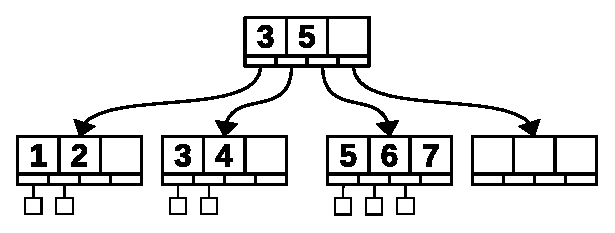
\includegraphics[width=\linewidth]{resources/made/a4_b_tree.eps}
                \end{figure}    
                \btreeSearchStepOne
            \end{block}
        \end{column}
    \end{columns}
\end{frame}
\begin{frame}
    \frametitle{B-Tree Operations - Search (Example)}
    \begin{columns}
        \begin{column}{.45\textwidth}
            \vspace{-1cm}
            \begin{block}{}
                \begin{itemize}
                    \item Due to \lstinline|b->keys[pos] != key|, we have to search in the node with index \lstinline|pos|. Where we repeat almost the same search process.
                    \item Since \lstinline|a[mid] < key| for the next 2 iterations, then \lstinline|lo = mid = 1|. But this time \lstinline|a[1] == key|, so we just return \lstinline|mid|.
                    \item Also, we have that \lstinline|b->keys[pos] == key|, so we \textbf{finally return \(1\)}.
                \end{itemize}
            \end{block}
        \end{column}
        \begin{column}{.6\textwidth}
            \vspace{-1cm}
            \begin{block}{}
                \begin{figure}[h!]
                    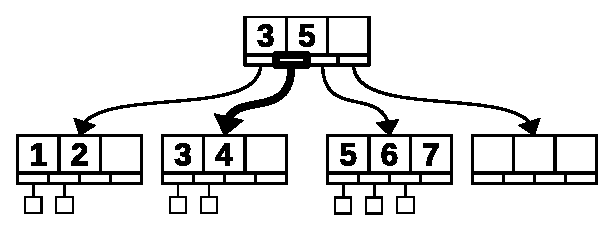
\includegraphics[width=\linewidth]{resources/made/a4_b_tree_searchstep2.eps}
                \end{figure}    
                \btreeSearchStepTwo
            \end{block}
        \end{column}
    \end{columns}
\end{frame}
\begin{frame}[t,allowframebreaks]
    \subsubsection{Insert node}
    \frametitle{B-Tree Operation - Insert Node}
    \begin{columns}
        \begin{column}{\textlecolumn}
            \begin{block}{}
                \begin{itemize}
                    \item Unlike all the types of trees that we've seen, in order to insert an element with it's key and value, we can't create a leaf node and insert it besides the other leaves of the tree, and if needed do some rotations in order to keep balance.
                    \item We can only insert the key into a existing Node, and keeping in mind the \emph{Branching factor} of the tree at all times by avoiding filling up the node elements to the upper bound.
                    \item Keeping the \emph{Branching factor} right is made by splitting of the nodes and then rotating around their \textbf{median key}.
                \end{itemize}
            \end{block}
        \end{column}
        \begin{column}{\textricolumn}
        \end{column}
    \end{columns}
    \begin{columns}
        \begin{column}{\textlecolumn}
            \begin{block}{}
                \begin{itemize}
                    \item The \lstinline|insert| operation mainly depends on the function \lstinline|insertInternal| which takes handles almost all of the important logic when we are inserting a new key in the tree.
                    \item The only case handled in the \lstinline|insert| operation if when we have split a node and need to create a new root to it points to the old and new nodes.
                \end{itemize}
            \end{block}
        \end{column}
        \begin{column}{\textricolumn}
        \end{column}
    \end{columns}
    \btreeInsert
    \begin{columns}
        \begin{column}{\textlecolumn}
            \begin{block}{}
                \begin{itemize}
                    \item The \lstinline|insertInternal| function starts by getting the position of the key in the node by using \lstinline|searchKey|, the same function that in the \lstinline|search| operation.
                    \item This to first check if the key is already in the node. 
                    \item And since the \lstinline|searchKey| function gives us the smaller index \(i\) such that for a node \(n\) and key \(k\) to insert: \(k \leq n.keys\left[i\right]\).
                    \item If we are in a leaf we can insert the key directly by moving the memory of the keys in the array of the node by 1 position:
                \end{itemize}
            \end{block}
        \end{column}
        \begin{column}{\textricolumn}
        \end{column}
    \end{columns}
    \btreeInsertInternalPartOne
    \vspace{-1cm}
    \begin{columns}
        \begin{column}{\textlecolumn}
            \begin{block}{}
                \begin{itemize}
                    \item Otherwise we will call recursively \lstinline|insertInternal| until we reach a leaf that we can insert the key.
                \end{itemize}
            \end{block}
        \end{column}
        \begin{column}{\textricolumn}
        \end{column}
    \end{columns}
    \btreeInsertInternalPartTwo
    \begin{columns}
        \begin{column}{\textlecolumn}
            \begin{block}{}
                \begin{itemize}
                    \item Then, we will check if the number of keys in the node doesn't overflow the \(2\alpha - 1\) upper limit.
                    \item In case of overflow, we will calculate the median key of the node, and pass it to \lstinline|insert| via an argument by reference.
                    \item Then, it'll create a new node with the elements, keys and sub-trees to the right of the median key.
                    \item Also setting node information like the number of keys, and is it's a leaf.
                    \item Otherwise, if there's no overflow, just return 0.
                \end{itemize}
            \end{block}
        \end{column}
        \begin{column}{\textricolumn}
        \end{column}
    \end{columns}
    \btreeInsertInternalPartThree
    \vspace{-1cm}
    \begin{columns}
        \begin{column}{\textlecolumn}
            \begin{block}{}
                \begin{itemize}
                    \item And thus, completing the \lstinline|insert| operation.
                    \item Since we had to access nodes all the way until a leaf, and re-balance a bunch of the nodes in the worst scenario.
                    \item The operation will take only \(O\left(log_\alpha \frac{n + 1}{2}\right)\) of CPU processing and  \(O\left(h\right)\) of disk accesses.
                    \item Which is fast, but there's tree that are faster in this process, mainly in the disk access.
                \end{itemize}
            \end{block}
        \end{column}
        \begin{column}{\textricolumn}
        \end{column}
    \end{columns}
\end{frame}
\begin{frame}
    \subsubsection{Destroying a B-Tree}
    \frametitle{B-Tree Operation - Destroying a B-Tree}
    \begin{columns}
        \begin{column}{\textlecolumn}
            \begin{block}{}
                \begin{itemize}
                    \item We just iter through each node recursively, freeing the leaves first and then the inner nodes all the way to the \emph{Root} of the tree.
                \end{itemize}
                \btreeDestroy
            \end{block}
        \end{column}
        \begin{column}{\textricolumn}
        \end{column}
    \end{columns}
\end{frame}
\begin{frame}
    \subsection{Secondary Memory Access}
    \frametitle{B-Tree Secondary Memory Access}
    \begin{columns}
        \begin{column}{.7\textwidth}
            \begin{block}{}
                \begin{itemize}
                    \item Fairly good for storing data in external memory in comparison to height, weight or search trees.
                    \item The limit of \(2\alpha - 1\) help us by forcing that each size node will be optimized.
                    \item But, this limit also make that if we need to re-balance the tree the 
                        operation will take \(\Theta\left(\alpha log n\right)\), updating all the split nodes.
                    \item This operation doesn't affect much in main memory, but in secondary memory where each reading can take longer time due to the technology available we might run in multiple problems of efficiency.
                \end{itemize}
            \end{block}
        \end{column}
        \begin{column}{.35\textwidth}
            \begin{block}{}
                \begin{figure}[h!]
                    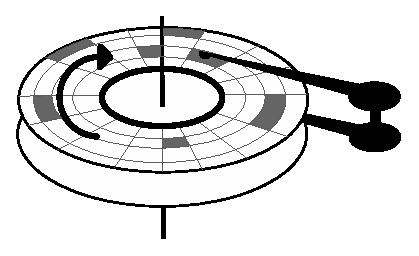
\includegraphics[width=\linewidth]{resources/made/external_storage_wblocks.eps}
                    \caption{External storage with the sectors to access highlighted}
                    \label{external_storage_wblocks}
                \end{figure}
            \end{block}
        \end{column}
    \end{columns}
\end{frame}
   
%\begin{frame}
%    \section{(a,b)-Tree}
%    \frametitle{(a,b)-Tree}
%\end{frame}
%\begin{frame}
%    \subsection{Properties}
%    \subsubsection{Keys and Sub-trees}
%    \frametitle{(a,b)-Tree Properties - Keys and Sub-trees}
%\end{frame}
%\begin{frame}
%    \subsubsection{Height}
%    \frametitle{(a,b)-Tree Properties - Height}
%\end{frame}
%\begin{frame}
%    \subsection{Structure}
%    \frametitle{(a,b)-Tree Properties - Structure}
%\end{frame}
%\begin{frame}
%    \subsection{Operations}
%    \frametitle{(a,b)-Tree Properties - Operations}
%\end{frame}

\begin{frame}
    \section{Bibliography}
    \frametitle{Bibliography}   
    \nocite{*}
    \printbibliography[heading=none]
\end{frame}

\end{document}
